\chapter{Elastic Structures}
\label{ch:elastic_structures}
\graphicspath{{elastic_structures/fig/}}

Elastic behaviour is ubiquitous in both nature and engineering applications, and in many cases, they exhibit multistability and can reversibly change between different configurations.
Such systems have wide-ranging potential applications, such as deployable structures \cite{Filipov2015,Zhai2018,Zareei2020}, micro-electromechanical systems \cite{Felton2014,Ko2017}, robotics \cite{Kwok2014,Chen2018a,Gorissen2020,Currier2020,Tang2020}, and energy absorption \cite{Shan2015,Bertoldi2017a}.
These are often complex structures, but the multistable behaviour is usually derived from simple elements, such as buckled beams or surfaces, and elastic joints or creases.
In this chapter various types of multistable elastic structures will be outlined, along with some of the recent and ongoing research on this topic.



\section{Buckling}
Buckling is a sudden change of shape that occurs when a structure is subject to compressive strain.
Generally, this is an undesired effect that is associated with structural failure and can have severe consequences, particularly if it occurs in buildings or other infrastructure.
Therefore, fields such as structural engineering utilise a range of techniques to prevent buckling and ensure the stability of structures.
However, recently there has been significant interest in exploiting buckling transitions to develop flexible devices and structures that can reversibly transform from an undeformed state to a buckled state, or between two different buckled states.
Some key examples will be discussed here.

The most basic, and perhaps most versatile, buckled system is that of a column or thin beam under compression.
This is possible to be monostable or bistable, depending upon the strain applied and angles at which the end points are held.
Previous research has extensively surveyed the stability of the states under different sets of parameters \cite{Wan2020}.
This can therefore be applied to understand the behaviour of more complex structures constructed from simple beam elements.

\begin{figure}[htb]
  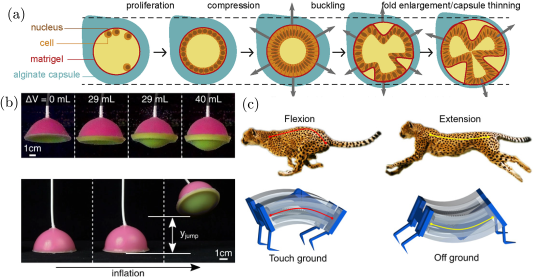
\includegraphics[width=\textwidth]{buckling.png}
  \caption{
    (a) Schematic showing how the growth of a membrane of cells can lead to buckling and the formation of folds.
        Adapted with permission from \cite{Trushko2020}.
    (b) A soft jumper that uses the snap-through buckling of a spherical shell upon inflation.
        Adapted with permission from \cite{Gorissen2020}.
    (c) A cheetah-inspired soft actuator for robotic movement.
        A central bistable linkage is used in combination with with inflatable channels to change states.
        Adapted with permission from \cite{Tang2020}.
  }
  \label{fig:es-buckling}
\end{figure}

While global buckling modes are typically observed in thin beams, surfaces and thin shells can exhibit local buckle through the formation of dimples on the surface.
This is generally undesired in engineering applications, such as containers or rockets, and is important to understand how it occurs in order to prevent and control structural failure.
The size of disturbances that are required in order to buckle both cylindrical and spherical shells under strain have been investigated by applying probing forces \cite{Virot2017,Hutchinson2018}.
In addition, various works have investigated the effect of imperfections, which can significantly reduce resistance to buckling \cite{Deml1997,Hutchinson2018}.
These findings highlight the precise manufacturing that is required to ensure that buckling cannot occur.

The buckling of surfaces and membranes also plays an important role in various biological functions.
One case is in the formation of folded structures of cell layers, which are essential in many anatomical structures such as glands or crypts.
Buckling is a possible mechanism for the formation of these structures.
For example, it can be caused by the growth of cells when constrained by a surface \cite{Nelson2011,Trushko2020}, \cref{fig:es-buckling}(a).
Many of these biological membranes, such as lipid bilayers, are a liquid surface that can redistribute to reduce local stress, but these too can buckle.
An example of this is the budding of cell membranes, where the binding of curved structures to the membrane can result in stress that causes the surface to buckle \cite{Lenz2009}.
Furthermore, it is possible to use the onset of buckling to measure the mechanical properties of cells \cite{Evans1983}.

% [[In small scale systems, such as in cells, capillary forces of liquids can become significant and deform elastic structures.]]
% [[This is known as elasto-capillarity and involves a competition between surface tension deforming the structure, and the elastic force restoring it.]]
% [[When the surface tension wins out it can cause buckling to occur \cite{Andreotti2011}.]]
% [[Elasto-capillarity can cause cell membranes to deform and engulf droplets \cite{Kusumaatmaja2011}, which is another cause of cell budding.]]
% [[This has also been applied to droplets on substrates with different shapes, which then fold and engulf the droplets into different shapes \cite{Roman2010}.]]
% [[Elasto-capillarity can also lead to the collapse of surfaces and tubes \cite{Roman2010,Emery2021}, as well as the buckling and coilling of elastic rods constrained within a droplet \cite{Elettro2017}.]]

An area where buckling can be highly beneficial is in the development of soft actuators for robotics.
In contrast to traditional robotic motion, soft actuators can provide simpler systems that are lighter, less prone to failure, and safer around humans.
Using buckling instabilities it is possible to amplify actuation of these soft structures, causing large, sudden displacements which can be used for propulsion.
For example, bistable beams have been used to propel swimming robots \cite{Chen2018a}, and the snap-through of spherical shells has been used for inflatable jumpers \cite{Gorissen2020}, shown in \cref{fig:es-buckling}(b).
Buckling can further be used to emulate biological behaviour such as swimming fish \cite{Currier2020}, and the galloping of cheetahs \cite{Tang2020}, \cref{fig:es-buckling}(c).
Finally, bistable structures have been used in pneumatic soft grippers that can be pressurised to pick up objects and continue to hold them even when the pressure is released \cite{Yang2015,Faber2020}.



\section{Buckled mesostructures}\label{sec:es-mesostructures}
The class of elastic structures that will primarily be investigated in this thesis are known as 3D buckled mesostructures.
These are produced as a flat pattern which buckles under a compressive strain to form a three-dimensional structure.
Typically, this is carried out by binding the structure at various points to a pre-stretched substrate, which is then released, compressing the structure.
This provides a simple method for fabricating complex structures, and can be used to create structures down to the microscale.
These have been investigated for applications such as flexible electronics \cite{Fu2018}, microelectromechanical systems \cite{Fu2018,Ning2018}, biomedical devices \cite{McCracken2017,Yan2017}, and microrobotics \cite{Yan2017}.

Many works have investigated the resultant three-dimensional structures for various different precursor patterns.
Simple patterns may consist of a single ribbon or a connected grid of ribbons with periodic bonding sites, in which case the ribbons will buckle into a wavy structure, \cref{fig:es-mesostructures}(a).
Or if the ribbons are curved, they can twist into helical coil shape when buckled \cite{Xu2015}.
By connecting these ribbons together in complex networks, it is possible to create multilevel, buckled designs.
Generally, these structures will buckle up fully.
However, if the adhesive force to the substrate is strong ,such as for very small scale structures, it may remain attached to the substrate in various locations \cite{Liu2019}.

\begin{figure}[htb]
  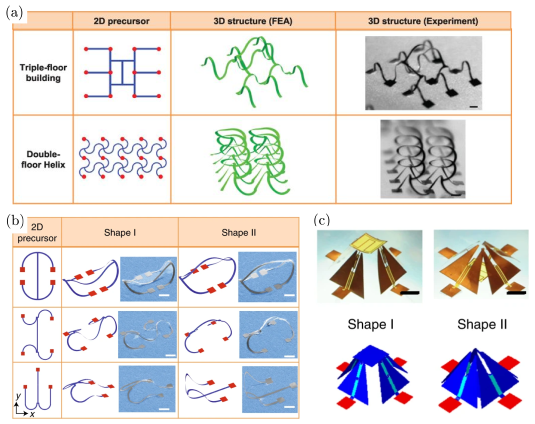
\includegraphics{mesostructures.png}
  \label{fig:es-mesostructures}
  \caption{
    (a) Buckled mesostructures with patterns that produce multilevel structures.
        Adapted with permission from \cite{Xu2015}.
    (b) Multistable mesostructures that can each take two different buckled states.
        Adapted with permission from \cite{Fu2018}.
    (c) A multistable mesostructure with a radio-frequency antenna on top.
        In shape 1 the antenna is free to transmit, but in state 2 it is blocked.
        Adapted with permission from \cite{Silverberg2014}.
  }
\end{figure}

It is possible for some mesostructures to buckle into multiple different stable configurations, such as those seen in \cref{fig:es-mesostructures}(b).
However, these structures are limited and it may be difficult to obtain more than a single state in practice.
This multistability can be enhanced by incorporating origami-like creases into the structure where it can more easily bend \cite{Fu2018}.
This greatly increases the variety of structures with multiple stable stables and allows greater control over which states are stable.
This can be utilised to create switchable devices, such as an antenna that can transmit in one configuration, but is shielded in another, as depicted in \cref{fig:es-mesostructures}(c).

A number of different approaches have been suggested in order to obtain these different states.
Fu et al. \cite{Fu2018} discovered a method of producing different shapes by controlling the release of the underlying substrate over time.
By independently releasing the substrate in different directions they were able to obtain structures with three separate states.
In this approach, the available states are limited to those that are spontaneous under buckling.
Park et al. \cite{Park2019} were able to control the shape of the structure over time by dissolving a constricting film.
However, this approach is irreversible and the possible shapes are limited.
Furthermore, they suggested a method for keeping the mesostructures buckled after removing from the substrate, by interlocking parts of the structure to keep it in place.
A different approach has been considered by Hao et al. \cite{Hao2020}.
Instead of using a stretched substrate, they used structures made from hydrogels which swell, causing the structure to buckle.
They were able to control the buckling to obtain various stable configurations by preswelling parts of the structure.

Despite these methods for creating multiple stable states, reconfigurability after the structure is created has largely remained unaddressed.
An approach addressing this problem will motivate later work in \cref{ch:mesostructures,ch:origami_ribbon}.



\section{Mechanical metamaterials}\label{sec:es-metamaterials}
Although we focus primarily upon buckled mesostructures in this thesis, it is worth considering the related, and popular topic of mechanical metamaterials.
These are materials that have properties defined by their structure and not the properties of the constituent material.
They can show a variety of interesting and unusual properties such as negative Poisson ratio (auxetic materials) \cite{Bertoldi2017,Bertoldi2017a}, where the material expands (or contracts) in all directions simultaneously, or negative compressiblity \cite{Nicolaou2012,Lakes2001}, where the material contracts under a tensile force.
There are many different types of mechanical metamaterials, but each of which is typically made up of a repeating pattern of simple elements, such as beams or hinges \cite{Bertoldi2017}.
If these individual elements are multistable by undergoing a buckling transition, then the metamaterial itself will be multistable.

Some metamaterials can have large numbers of elements that buckle at once under compression or tension \cite{Che2017,Bertoldi2017a}.
An example is the 3D elastomeric structure shown in \cref{fig:es-metamaterials}(a), where the array of holes can collectively buckle, resulting in a highly non-linear compressive behaviour with a negative Poisson ratio \cite{Bertoldi2010,Florijn2014,Bertoldi2017a,Medina2020}.
Similar structures with buckling beams have also been proposed for energy absorption and storage \cite{Shan2015,Che2017,Bertoldi2017a,Giri2021}.
These have advantages over traditional materials used for collision protection because they can easily unbuckled and reused.
The structures can also exhibit hysteresis loops under cyclic loading and unloading, and so can be used for dissipating energy and damping vibration \cite{Bertoldi2017a}.
The order of buckling in these structures is unpredictable because each cell is identical and will depend upon manufacturing imperfections, but this can be controlled by varying the thickness of the bistable beams \cite{Che2017,Giri2021}.

Energy absorbing metamaterials are generally constructed in arrays, with rows of cells that buckle together, but not all at once.
However, for some metamaterials, the transition of one cell can destabilise neighbouring sections and lead to a cascade across the entire structure.
These are attractive for realising complex, self-deploying structures \cite{Zareei2020}.
The change of state occurs through transition waves that travel at a constant speed through the structure, behaving similarly to phase transitions observed in crystalline solids \cite{Jin2020}.
The transition waves can also be controlled and redirected by introducing defects into the periodic structure, as seen in \cref{fig:es-metamaterials}(b).

% Opposite to this are mechanical metamaterials are able to support local multistability by the buckling of individual elements.
% These structures can be programmed to set material properties such as stiffness \cite{Silverberg2014,Florijn2014,Chen2021}.
% For example, a metamaterial containing holes, similar to that in \cref{fig:es-metamaterials}(a), can be laterally confined at chosen locations.
% As this number of confined locations is increased, the mechanical response becomes more and more non-monotonic and hysteretic \cite{Florijn2014}.
% Another metamaterial has been demonstrated that is constructed of elements that contain a stopper that buckles up or down to block or allow compression \cite{Chen2021}.
% These can be individually switched between the two states on-demand, using a magnetic force.
% Two- or Three-dimensional arrays can therefore be constructed to produce a metamaterial with a reprogrammable and fine-tunable stiffness.

In addition to exhibiting interesting behaviour under compression, metamaterials can also be used to create multifunctional structures that morph into a variety of different configurations \cite{Shim2012,Haghpanah2016,Overvelde2017,Iniguez-Rabago2019,Zareei2020}.
One approach consists of tessellating prismatic structures with flexible hinges, \cref{fig:es-metamaterials}(c), which are able to change into a large variety of different shapes thanks to their 3D structure \cite{Overvelde2017,Iniguez-Rabago2019}.
These can be used to create structures that modify their shape and behaviour based upon changing environments, and be used to perform multiple tasks.
These structures are able to remain in the different configurations without an applied force because of multiple stable states resulting from the buckling of the rigid faces \cite{Iniguez-Rabago2019}.
A similar idea is seen in \cite{Shim2012}.
Here, the authors design a metamaterial that consists of an elastic spherical sphere that can undergo transformation from a large sphere with a relatively open surface to a small sphere with a dense surface.
Such a device could offer reversible encapsulation functionality in order to transport small quantities of substances.

\begin{figure}[htb]
  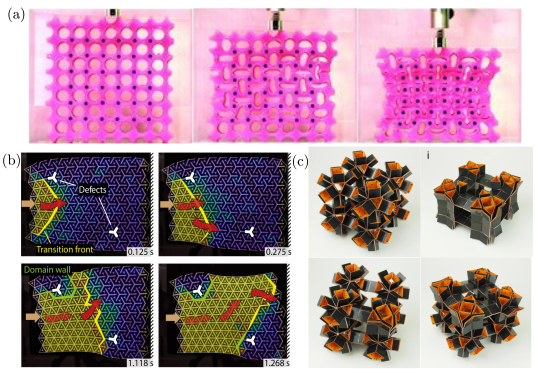
\includegraphics{metamaterials.png}
  \label{fig:es-metamaterials}
  \caption{
    (a) An elastic metamaterial with holes that buckle under compression.
        Adapted with permission from \cite{Overvelde2012}.
    (b) A transition wave through an auxetic metamaterial that is redirected by lattice defects.
        Adapted with permission from \cite{Jin2020}.
    (c) A 3D prismatic metamaterial that is able to reconfigure into a variety of stable states.
        Adapted with permission from \cite{Iniguez-Rabago2019}.
  }
\end{figure}



\section{Origami}
Origami structures are a specific type of mechanical metamaterial that have garnered considerable attention in particular.
They consist of a network of rigid flat surfaces joined by creases that are free to bend, which enables simple two-dimensional surfaces to form complex three-dimensional structures.
Origami is used for both artistic purposes and engineering applications, largely for its ability to produce strong, but light structures and materials \cite{Lv2014}.
One particularly useful class of origami structures are those that can fold from a flat surface, known as flat foldable, and are therefore easy to produce.
The simple reconfigurability of flat foldable structures also makes them suitable for deployable structures, such as solar panels for satellites \cite{Miura1985,Evans2015}.

By considering elastic folds with an optimal angle and allowing some bending of the rigid faces, many origami structures are found to be multistable.
Indeed, one of the most basic components of origami (vertices of four creases) is multistable \cite{Waitukaitis2015} and that these can be tiled to create large reconfigurable structures.
One such tiled structure is the Miura-ori pattern, \cref{fig:es-origami}(b), which is well known for its ability to unfold from a compact structure to a flat surface in a single motion as a result of a negative Poisson ratio \cite{Miura1985,Evans2015}.
For this usage, the structure is elastically monostable and therefore requires actuation to remain in a deployed state.
Bistability has been observed, however, through the inversion of singular cells of the Miura-ori pattern to create ``pop-through defects''.
These can be introduced to programmatically modify the stiffness of the structure, while remaining completely reversible \cite{Silverberg2014}.

Beyond simple sheets, origami can be used to produce three-dimensional structures.
For example, by stacking origami sheets, cellular metamaterials can be produced that are auxetic or can be used for impact energy absorption \cite{Fang2017,Harris2021}.
The behaviour is then easily tunable by modifying the underlying two-dimensional fold pattern.
Alternatively, the origami sheets can be curved and turned into tubes and cylinders \cite{Filipov2015,Zhai2018}.
These tubes are then able to easily extend and collapse simply by deforming the end, providing another useful approach for realising deployable structures.

Kirigami is a variation of origami whereby cuts are introduced into the surface in addition to folding.
This allows for structures with greater flexibility and additional stable states, with each end of a cut able to take one of two different states \cite{Sadik2021}.
The introduction of cuts also allows the structure to deform and buckle under compression \cite{Brighenti2005}, which has been exploited to create a variety of simple actuators that rotate or lift \cite{Dias2017}.

\begin{figure}
  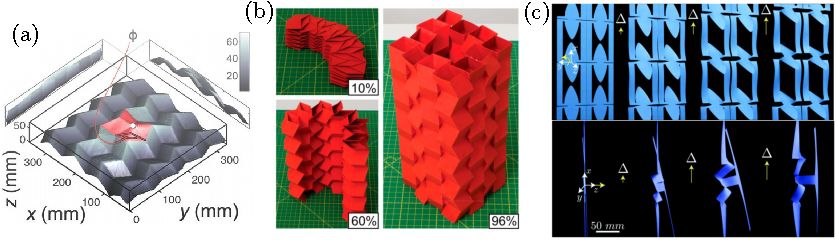
\includegraphics[width=\textwidth]{origami.pdf}
  \caption{
    (a) A Miura-ori pattern with a pop-through defect (red) that alters the stiffness of the structure. 
        Adapted with permission from \cite{Silverberg2014}.
    (b) A combination of 12 origami tubes that deploy to produce an enclosed structure.
        Adapted with permission from \cite{Filipov2015}.
    (c) Two kirigami actuators that rotate and lift, respectively, when extended.
        Adapted with permission from \cite{Dias2017}.
  }
  \label{fig:es-origami}
\end{figure}



\section{Energy landscapes applied to elastic structures}
Recently there has been increasing interest in using energy landscape methods to investigate multistable elastic structures \cite{Iniguez-Rabago2019,Medina2020,Silverberg2015,Zhai2018,Hutchinson2018,Virot2017,Panter2019}.
Since these structures are primarily macroscopic, thermal effects are insignificant and are external forces are needed to reconfigure them instead.
Correspondingly, there is no need to investigate their statistical behaviour.
Instead, energy landscape analysis can be used to design structures, and to inform how best to reconfigure them.
% The latter being particularly important owing to the complex and highly non-linear pathways that these structures often have.

Perhaps the most common use of energy landscapes in the field is to determine the various states that a given structure can take for given structural parameters.
For example, this has been used in the study of some reconfigurable mechanical metamaterials.
Iniguez-Rabago et al. have looked into several shape-changing 3D prismatic structures \cite{Iniguez-Rabago2019}.
By varying just two of the fold angles they were able to produce a simplified landscape, shown in \cref{fig:es-landscapes}(a), displaying the stable regions of each of the structure's various states.
A similar survey was also carried out for the elastomeric metamaterial with cylindrical holes that buckles under compression \cite{Medina2020}.
To understand how it behaves when compressed, all of the possible states were identified at increasing levels of strain, \cref{fig:es-landscapes}(b).
Furthermore, by introducing slight imperfections to the structure they were able to identify which of the states are obtained upon experimentally deforming the system.

% The central building block for many multistable elastic structures are compressed beams, which are bistable.
% Energy landscape surveys have been performed for these to determine for what strain and angles the beam will take different states \cite{Wan2020}.
% The landscapes of such a beam are simple, yet important, owing to their many uses, for example in metamaterials that absorb energy under compression \cite{Shan2015}.
% For this, the buckling pathways have been studied to find the energy barrier and force curves.
% The barriers have also been modified by changing the thickness of the beams in the structure in order to control the order that they buckle \cite{Che2017,Giri2021}.

% Another multistable structure is the square twist, an auxetic structure made up of square and rhombus faces.
% This undergoes a bistable transition from an unfolded state to a folded state, during which the faces are required to bend.
% This structure has been studied in detail in \cite{Silverberg2015} where a minimum angle is identified for the rhombus faces that gives a bistable structure, and as the stiffness of the faces is increased, this critical angle reduces to zero.

Energy landscapes have also been utilised in the study of origami structures.
In particular, these have looked at the reconfiguration pathways, which are often complex and non-linear due to the folding through large angles.
% Some studies have sought to locate these to describe the functionality of the origami structures and the ease with which they can be refolded.
Silverberg et al. \cite{Silverberg2015} investigated the square twist structure which undergoes a bistable transition from an unfolded to folded state, during which the faces are required to bend.
They were able to identify how the rigidity and shape of the structure affected the transition pathway and its barrier, and thereby how they could be tuned for specific applications.
Another use of the pathway is demonstrated for an origami cylinder \cite{Zhai2018}, which is easily deployable as a result of the small energy barrier.
In this case, the MEP causes the cylinder to first extend beyond its deployed state before returning.
Therefore, the structure must take a different pathway when the deployed structure is placed under compression, ultimately resulting in a much higher energy barrier and stiffness.
However, in each of these cases the pathways have been identified by applying forces to the structure, rather than locating the MEP.

Recently, MEP methods have also enabled the identification of completely rigid folding pathways in origami structures, even when crease bending energy is disregarded, such that there is no energy barrier between the unfolded and folded states.
By employing a pathway search algorithm that was fixed at the two end points with an energy that penalised any deviations from rigid folding, Zhou et al. were able to locate the rigid folding pathway for the Miura-ori pattern \cite{Zhou2023}.
A similar method could also be applied to other reconfigurable structures that are not necessarily multistable, as long as the two end states to be known.
% In the same study a bistable structure, the waterbomb base, is also considered, as well as a joined array of these structures.
% This time crease bending is considered in order to identify the energy barriers between the stable states, which turn out to be several orders of magnitude higher than the initial estimate.

In addition to providing information about desired reconfigurabilty, pathway analysis can be used to identify the failure modes of a system.
For example, the buckling of spherical and cylindrical shells under axial compression is hard to predict and depends strongly upon the size of any imperfections \cite{Hutchinson2018}.
However, by studying the energy barrier it is possible to identify how these imperfections affect the critical pressure before buckling occurs \cite{Hutchinson2018,Virot2017}.
Further work has also been undertaken to identify how the shape of the cylinders affects the structure of the energy landscape \cite{Panter2019}.
Panter et al. identified that short cylinders had simple funnelled landscapes, and long cylinders had complex landscapes with many more minima.
Furthermore, using the information about the initial buckling transition state, they were able to modify the distribution of the structure's thickness in order to maximise the energy barrier, and to control the energy landscape, reducing the number of states, \cref{fig:es-landscapes}(d).

\begin{figure}[htb]
  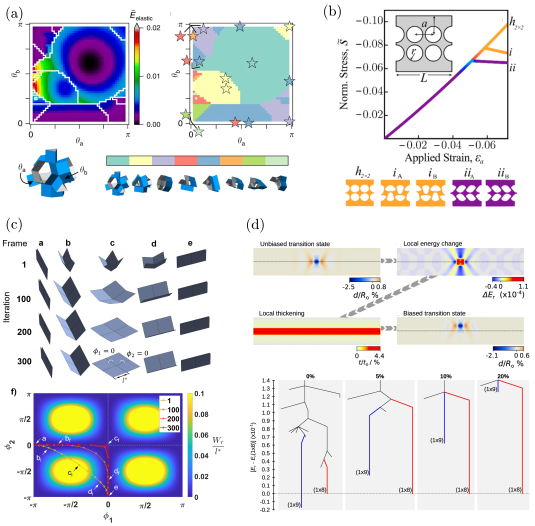
\includegraphics{landscapes.png}
  \label{fig:es-landscapes}
  \caption{
    Energy landscape methods applied to various elastic structures.
    (a) The landscape of a prismatic structure when varying two of the angles.
        The elastic energies of each configuration are shown on the left, and the basins of attraction for each state are on the right.
        Adapted with permission from \cite{Iniguez-Rabago2019}.
    (b) The stable states of a $2\times2$ holar metamaterial at different values of the compressive strain.
        Adapted with permission from \cite{Medina2020}.
    (c) Identifying the rigid folding pathway of a Miura-ori vertex using an NEB pathway.
        The top shows snapshots along the pathway as it is optimised.
        At the bottom the 2D energy landscape is shown.
        The pathway is refined towards the rigid folding pathway where the energy is zero.
        Adapted with permission from \cite{Zhou2023}.
    (d) Using information about the transition state of the buckling of a cylinder to alter the buckling behaviour.
        The top shows how the thickness is increased where the bending energy of the transition state is locally higher, resulting in an altered transition state.
        The bottom shows that, as the thickness is increased, the landscape changes and a low energy state is suppressed.
        Adapted with permission from \cite{Panter2019}.
  }
\end{figure}
